\documentclass{standalone}
\usepackage[utf8]{inputenc}
\usepackage[T1]{fontenc}

\usepackage[margin=1in]{geometry}
\usepackage{tikz-qtree}
\usetikzlibrary{shadows,trees}
\begin{document}
\tikzset{font=\small,
level distance=.8cm,
every node/.style=
    {color=white,
    rectangle,rounded corners,
    align=center,
    text = black
    },
edge from parent/.style=
    {draw=blue,
    thick
    }}

\centering
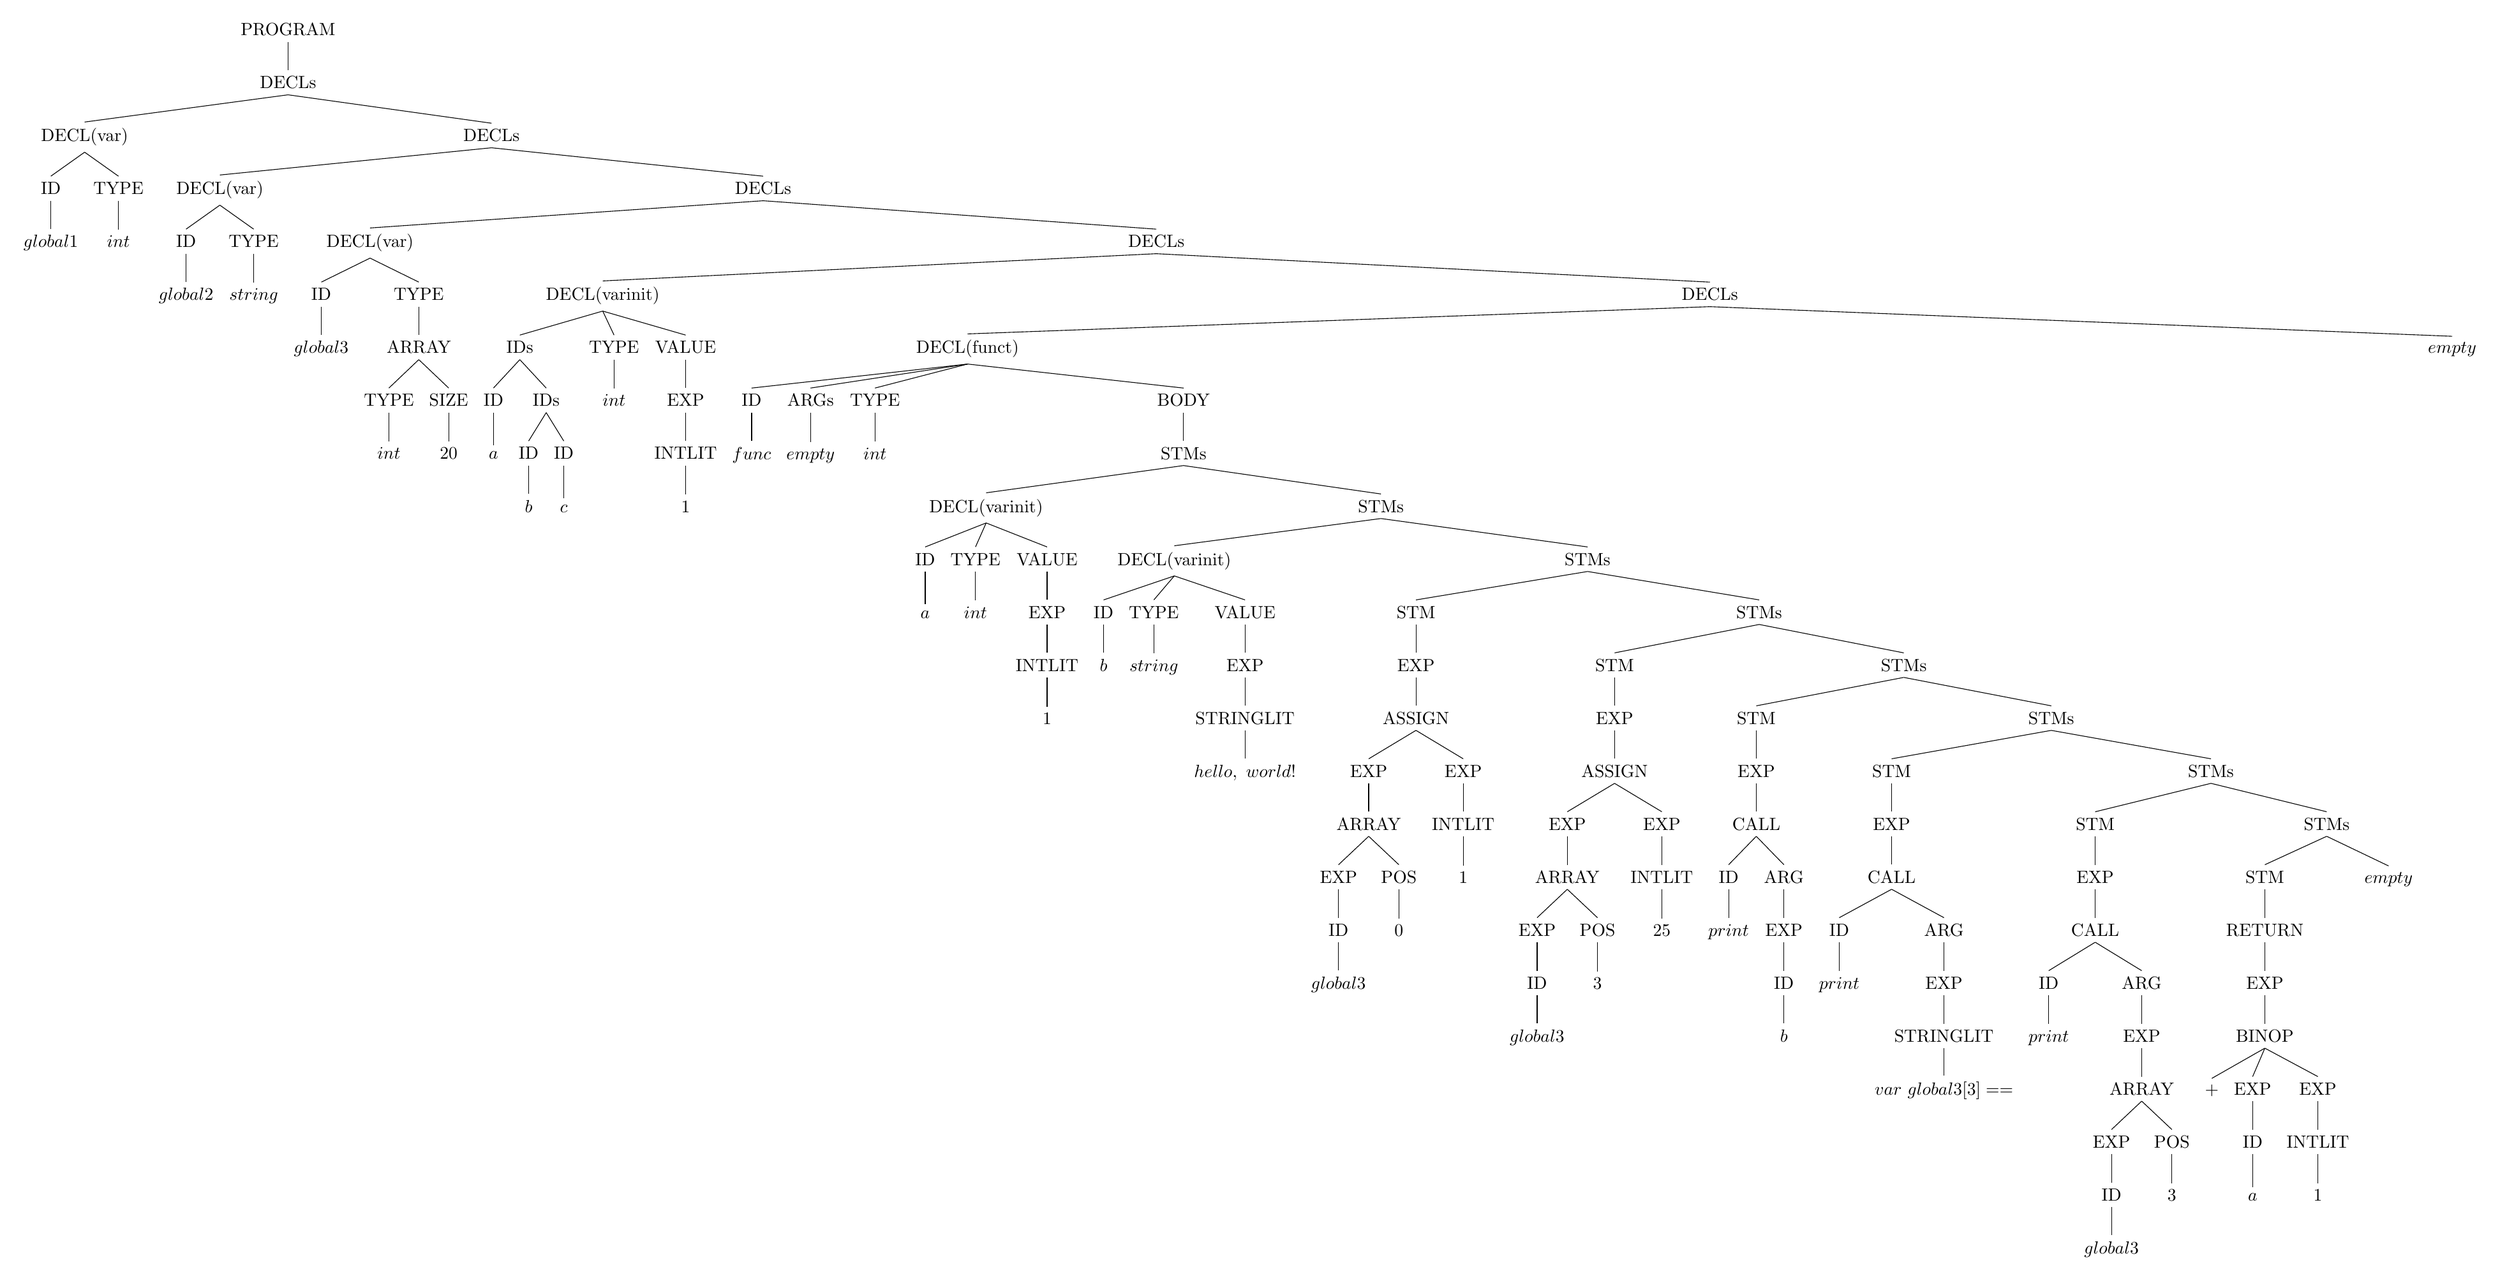
\begin{tikzpicture}
\Tree [.PROGRAM
[.DECLs [.DECL(var) [.ID $global1$ ][.TYPE $int$ ]
]
[.DECLs [.DECL(var) [.ID $global2$ ][.TYPE $string$ ]
]
[.DECLs [.DECL(var) [.ID $global3$ ][.TYPE [.ARRAY [.TYPE $int$ ]
[.SIZE $20$ ] ]]
]
[.DECLs [.DECL(varinit) [.IDs [.ID $a$ ] [.IDs [.ID $b$ ] [.ID $c$ ]]
]
[.TYPE $int$ ]
[.VALUE [.EXP [.INTLIT $1$ ] ]
] ]
[.DECLs [.DECL(funct) [.ID $func$ ] [.ARGs $empty$ ] [.TYPE $int$ ]
[.BODY [.STMs [.DECL(varinit) [.ID $a$ ][.TYPE $int$ ]
[.VALUE [.EXP [.INTLIT $1$ ] ]
] ]
[.STMs [.DECL(varinit) [.ID $b$ ][.TYPE $string$ ]
[.VALUE [.EXP [.STRINGLIT $hello,\ world!$ ] ]
] ]
[.STMs [.STM [.EXP [.ASSIGN [.EXP [.ARRAY [.EXP [.ID $global3$ ] ]
[.POS $0$ ] ] ]
[.EXP [.INTLIT $1$ ] ]
] ]
]
[.STMs [.STM [.EXP [.ASSIGN [.EXP [.ARRAY [.EXP [.ID $global3$ ] ]
[.POS $3$ ] ] ]
[.EXP [.INTLIT $25$ ] ]
] ]
]
[.STMs [.STM [.EXP [.CALL [.ID $print$ ] [.ARG [.EXP [.ID $b$ ] ]
]
] ]
]
[.STMs [.STM [.EXP [.CALL [.ID $print$ ] [.ARG [.EXP [.STRINGLIT $var\ global3[3]==$ ] ]
]
] ]
]
[.STMs [.STM [.EXP [.CALL [.ID $print$ ] [.ARG [.EXP [.ARRAY [.EXP [.ID $global3$ ] ]
[.POS $3$ ] ] ]
]
] ]
]
[.STMs [.STM [.RETURN [.EXP [.BINOP $+$ [.EXP [.ID $a$ ] ]
[.EXP [.INTLIT $1$ ] ]
] ]
] ]
$empty$ ]
]
]
]
]
]
]
]
] ]
$empty$ ]
]
]
]
]
]
\end{tikzpicture}
\end{document}
